%%%%%%%%%%%%%%%%%%%%%%%%%%%%%%%%%%%%%%%%%
% Beamer Presentation
% LaTeX Template
% Version 1.0 (10/11/12)
%
% This template has been downloaded from:
% http://www.LaTeXTemplates.com
%
% License:
% CC BY-NC-SA 3.0 (http://creativecommons.org/licenses/by-nc-sa/3.0/)
%
%%%%%%%%%%%%%%%%%%%%%%%%%%%%%%%%%%%%%%%%%

%----------------------------------------------------------------------------------------
%	PACKAGES AND THEMES
%----------------------------------------------------------------------------------------

\documentclass[spanish]{beamer}

\mode<presentation> {

% The Beamer class comes with a number of default slide themes
% which change the colors and layouts of slides. Below this is a list
% of all the themes, uncomment each in turn to see what they look like.

%\usetheme{default}
%\usetheme{AnnArbor}
%\usetheme{Antibes}
%\usetheme{Bergen}
%\usetheme{Berkeley}
%\usetheme{Berlin}
%\usetheme{Boadilla}
%\usetheme{CambridgeUS}
%\usetheme{Copenhagen}
%\usetheme{Darmstadt}
%\usetheme{Dresden}
%\usetheme{Frankfurt}
%\usetheme{Goettingen}
%\usetheme{Hannover}
%\usetheme{Ilmenau}
%\usetheme{JuanLesPins}
%\usetheme{Luebeck}
%\usetheme{Madrid}
%\usetheme{Malmoe}
%\usetheme{Marburg}
%\usetheme{Montpellier}
%\usetheme{PaloAlto}
%\usetheme{Pittsburgh}
%\usetheme{Rochester}
%\usetheme{Singapore}
%\usetheme{Szeged}
\usetheme{Warsaw}

% As well as themes, the Beamer class has a number of color themes
% for any slide theme. Uncomment each of these in turn to see how it
% changes the colors of your current slide theme.

%\usecolortheme{albatross}
%\usecolortheme{beaver}
%\usecolortheme{beetle}
%\usecolortheme{crane}
%\usecolortheme{dolphin}
%\usecolortheme{dove}
%\usecolortheme{fly}
%\usecolortheme{lily}
%\usecolortheme{orchid}
%\usecolortheme{rose}
%\usecolortheme{seagull}
%\usecolortheme{seahorse}
%\usecolortheme{whale}
%\usecolortheme{wolverine}

%\setbeamertemplate{footline} % To remove the footer line in all slides uncomment this line
%\setbeamertemplate{footline}[page number] % To replace the footer line in all slides with a simple slide count uncomment this line

%\setbeamertemplate{navigation symbols}{} % To remove the navigation symbols from the bottom of all slides uncomment this line
}

\usepackage{graphicx} % Allows including images
\usepackage{booktabs} % Allows the use of \toprule, \midrule and \bottomrule in tables
\usepackage[utf8]{inputenc} % Para los tildes

\usepackage{babel}
\addto\shorthandsspanish{\spanishdeactivate{~<>}}

\logo{
\includegraphics[height=0.15in]{logo-mina-right.png}}

%----------------------------------------------------------------------------------------
%	TITLE PAGE
%----------------------------------------------------------------------------------------

\title[Robotito]{Programando robots jugando con el entorno}  % The short title appears at the bottom of every slide, the full title is only on the title page
\author[Gonzalo Tejera]{~Gonzalo Tejera\inst{1}}
\institute[FIng::UdelaR]{\inst{1} Instituto de Computación\\
Facultad de Ingeniería\\
Universidad de la República}
\date[MINA 2018]{Grupo MINA, 2018}

%\medskip
%\textit{john@smith.com} % Your email address

\begin{document}

\begin{frame}
\titlepage % Print the title page as the first slide
\end{frame}

\begin{frame}
\frametitle{Contenido} % Table of contents slide, comment this block out to remove it
\tableofcontents % Throughout your presentation, if you choose to use \section{} and \subsection{} commands, these will automatically be printed on this slide as an overview of your presentation
\end{frame}

\section{Introducción}
\begin{frame}
	\frametitle{Motivación}
	\begin{itemize}
		\item Robótica educativa.
		\item Pensamiento computacional.
	\end{itemize}
\end{frame}

\begin{frame}
	\frametitle{Definición de robot}
	\begin{itemize}
		\item Un robot industrial es un manipulador multifuncional programable, capaz de mover materias, piezas, herramientas o dispositivos	especiales, según trayectorias variables, programadas para realizar tareas diversas [RIA2011].
		\item Un robot inteligente es un robot del cual se espera que aprenda y ejecute tareas aún en ambientes cambiantes. Un robot inteligente es una máquina capaz de extraer información de su ambiente y usar ese conocimiento para moverse en forma segura cumpliendo un propósito y sentido [Arkin1998].
	\end{itemize}
\end{frame} 

\begin{frame}
	\frametitle{Robótica educativa}
	\begin{itemize}
		\item Un contexto de aprendizaje que se apoya en las tecnologías digitales e involucra a
		quienes participan en el \textbf{diseño y construcción} de creaciones propias, \textbf{primero
		mentales y luego físicas}, construidas con diferentes materiales y controladas por un
		computador [Fundación Omar Dengo, 2007].
		\item El conjunto de \textbf{actividades pedagógicas} que apoyan y fortalecen áreas específicas
		del conocimiento a través de la \textbf{concepción, creación, ensamble y puesta a punto}
		de robots [Robótica Educativa de México, 2009].
	\end{itemize}
\end{frame} 

\begin{frame} <presentation:0> % hide slide
	\frametitle{Ejemplos de robots}
	\begin{itemize}
		\item Cellulo
		\item KIBO
		\item MOSS
	\end{itemize}
\end{frame}

\begin{frame}
	\frametitle{Pensamiento computacional}
	\begin{itemize}
		\item Resolver problemas, diseñar sistemas y entender el comportamiento humano a través de conceptos de las ciencias de la computación [Wing, 2006].
		
		\item Es el proceso de pensamiento involucrado en la formulación de problemas y sus soluciones para que estas puedan ser representadas en una forma que pueda ser efectivamente procesada por una computadora [Wing, 2010].
	\end{itemize}
\end{frame}


\section{Contexto robótico}

\begin{frame}
\frametitle{Proyecto Butiá}
  \begin{columns}[T]
    \begin{column}{.33\textwidth}
    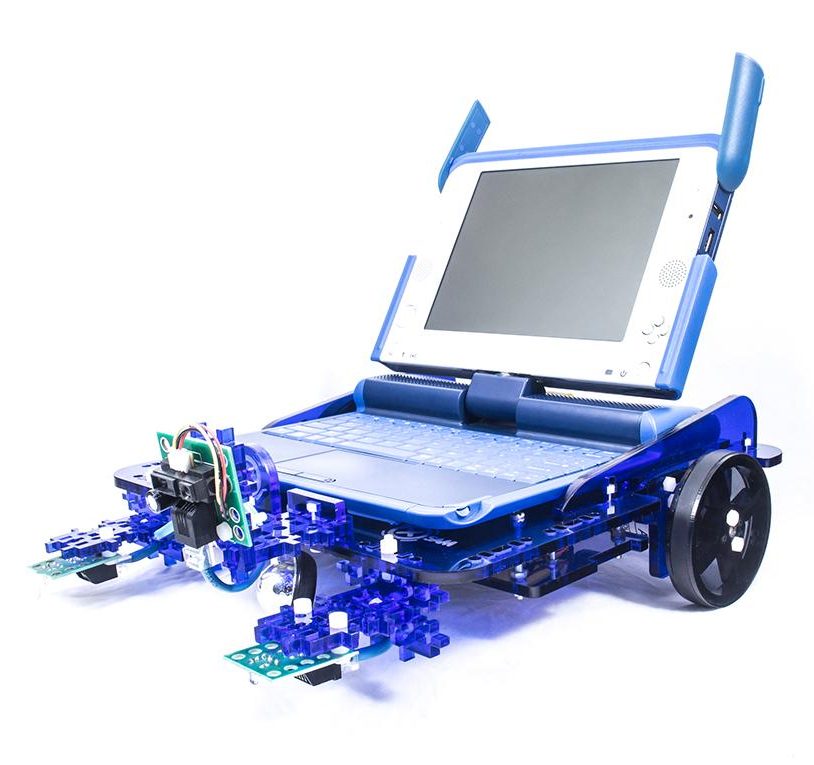
\includegraphics[width=\textwidth]{butia2.png}
    \end{column}
    \begin{column}{.33\textwidth}
    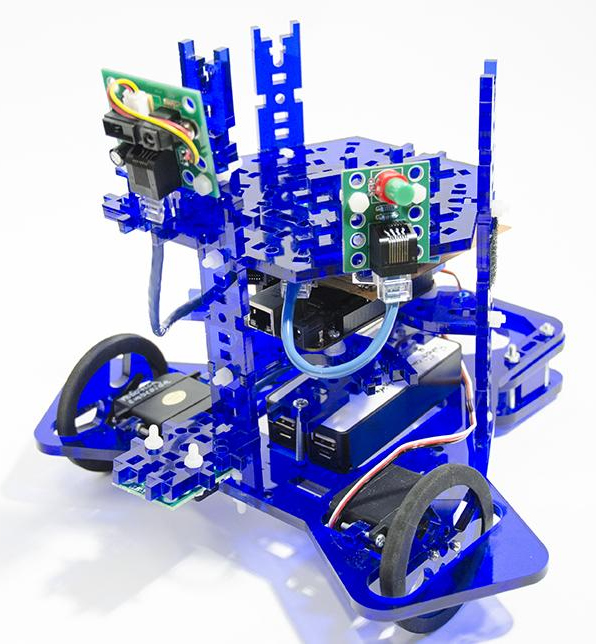
\includegraphics[width=\textwidth]{butia3.png}
    \end{column}
    \begin{column}{.33\textwidth}
    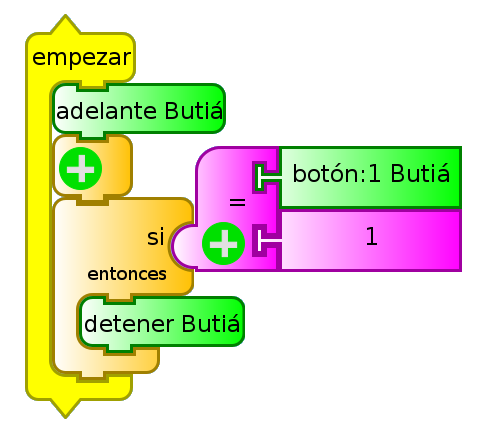
\includegraphics[width=\textwidth]{tortuga.png}
    \end{column}
  \end{columns}
\end{frame}

\begin{frame}
\frametitle{sumo.uy}
	\begin{itemize}
		\item Nueve categorías.
		\item 350 competidores.
		\item 120 equipos.
		\item Presentaciones.
		\item Talleres.
		\item Exposiciones.
	\end{itemize}
\end{frame}

\section{Proyecto}

\begin{frame}
	\frametitle{Objetivos}
	\begin{itemize}
		\item Desarrollar robot dotado en una serie de reglas para ser programable por el ambiente 
		\item Explorar qué habilidades cognitivas son necesarias para trabajar con esta propuesta. 
		\item Evaluar el impacto de la intervención en el desarrollo de las variables cognitivas analizadas. 
		\item Evaluar los aspectos motivacionales y de cooperación vinculados al juego con robots.
	\end{itemize}
\end{frame}

\begin{frame}
	\frametitle{Contexto}
	\begin{itemize}
		\item Financia ANII (Fondo Sectorial de Educación – Modalidad Inclusión Digital 2017).
		\item Desarrollan
		\begin{itemize}
			\item CICEA.
			\item Facultad de ingeniería.
		\end{itemize}
	\end{itemize}
\end{frame}

\begin{frame}
	\frametitle{Diseño de la investigación}
	\begin{center}
		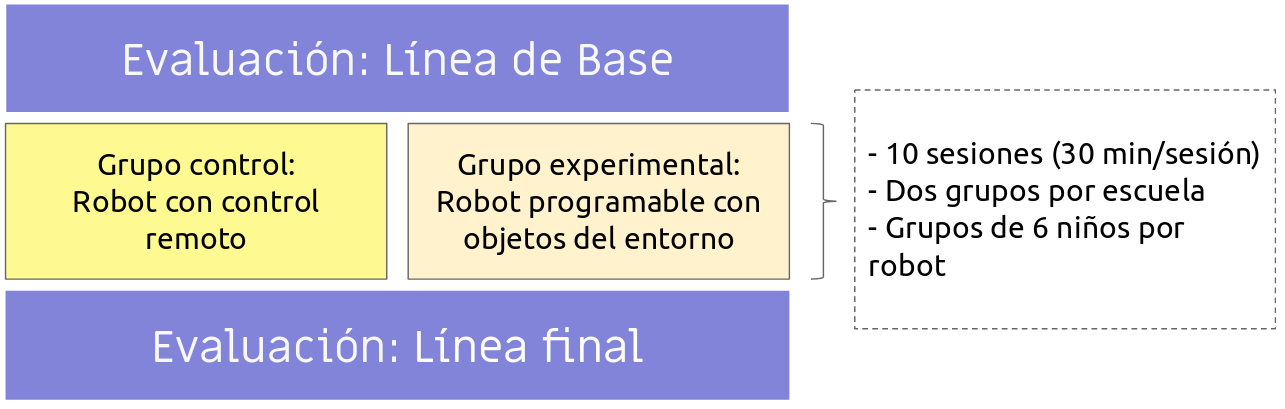
\includegraphics[width=\textwidth]{diseno-investigacion.png}
	\end{center}
\end{frame}

\begin{frame}
	\frametitle{Habilidades a evaluar}
	\begin{itemize}
		\item Pensamiento computacional
		\item Inteligencia fluida
		\item Memoria de trabajo no verbal
		\item Planificación
		\item Habilidad espacial, verbal y matemática.
	\end{itemize}
\end{frame}

\begin{frame}
	\frametitle{Prototipos}
	\begin{itemize}
		\item Faros
		\item Distancia a objetos
		\item Color de los objetos
	\end{itemize}
\end{frame}

\begin{frame}
	\frametitle{Prototipo 1}
  \begin{columns}[T]
  	\begin{column}{.5\textwidth}
  		\vspace{1em}
		\begin{itemize}
			\item Omni-direccional
			\item Sensores de distancia
			\item Campos repulsores.
		\end{itemize}
  	\end{column}
  	\begin{column}{.5\textwidth}
		\begin{center}
			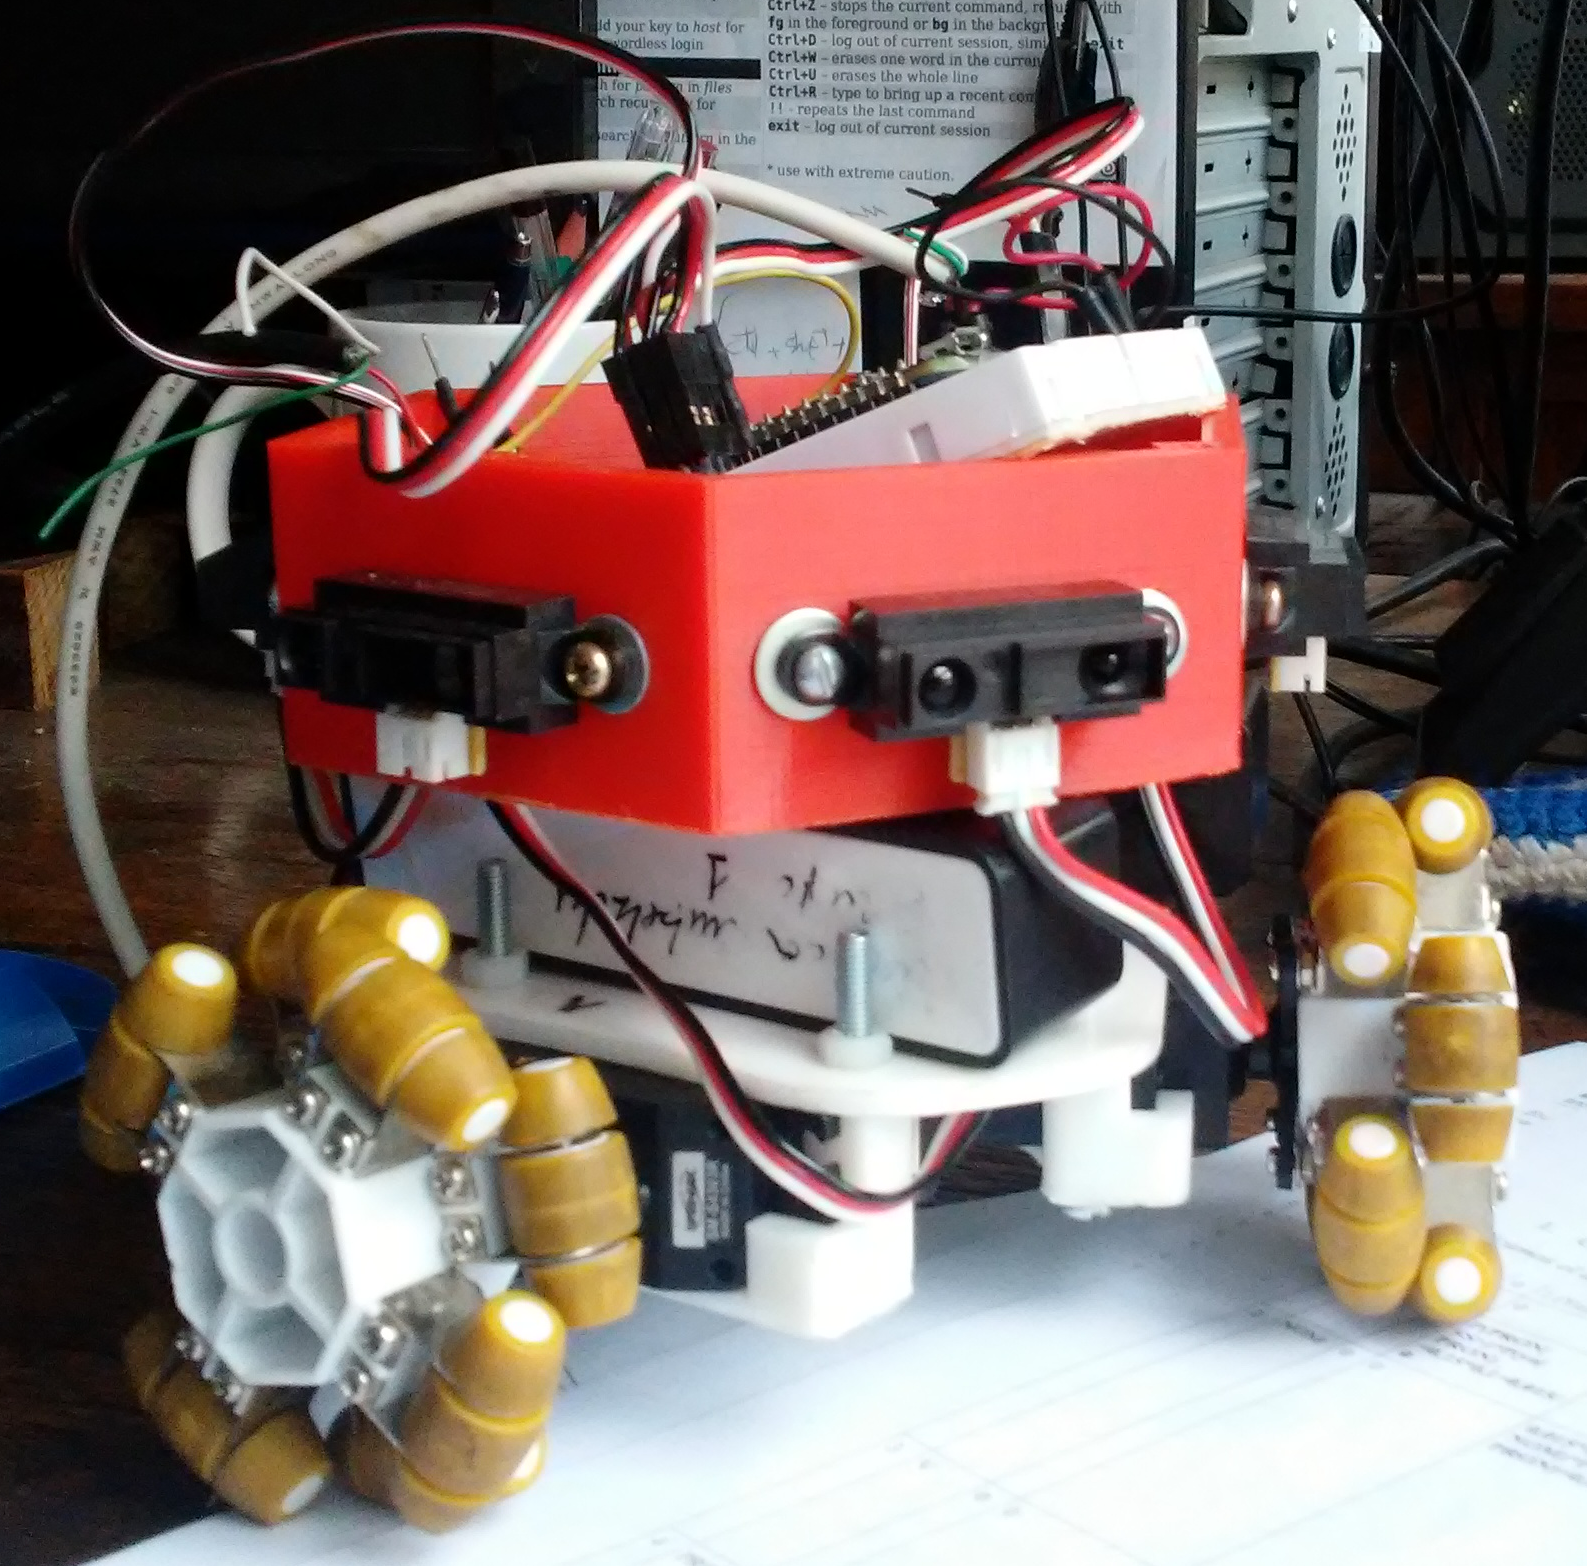
\includegraphics[width=\textwidth]{robotito.png}
		\end{center}
  	\end{column}
  \end{columns}
\end{frame}

\begin{frame}
	\frametitle{Prototipo 2-4}
	\begin{columns}[T]
		\begin{column}{.5\textwidth}
			\vspace{1em}
			\begin{itemize}
				\item Omni-direccional
				\item Sensores de distancia y de color
				\item Campos atractores y patrones fijos basados en color.
			\end{itemize}
		\end{column}
		\begin{column}{.5\textwidth}
			\begin{center}
				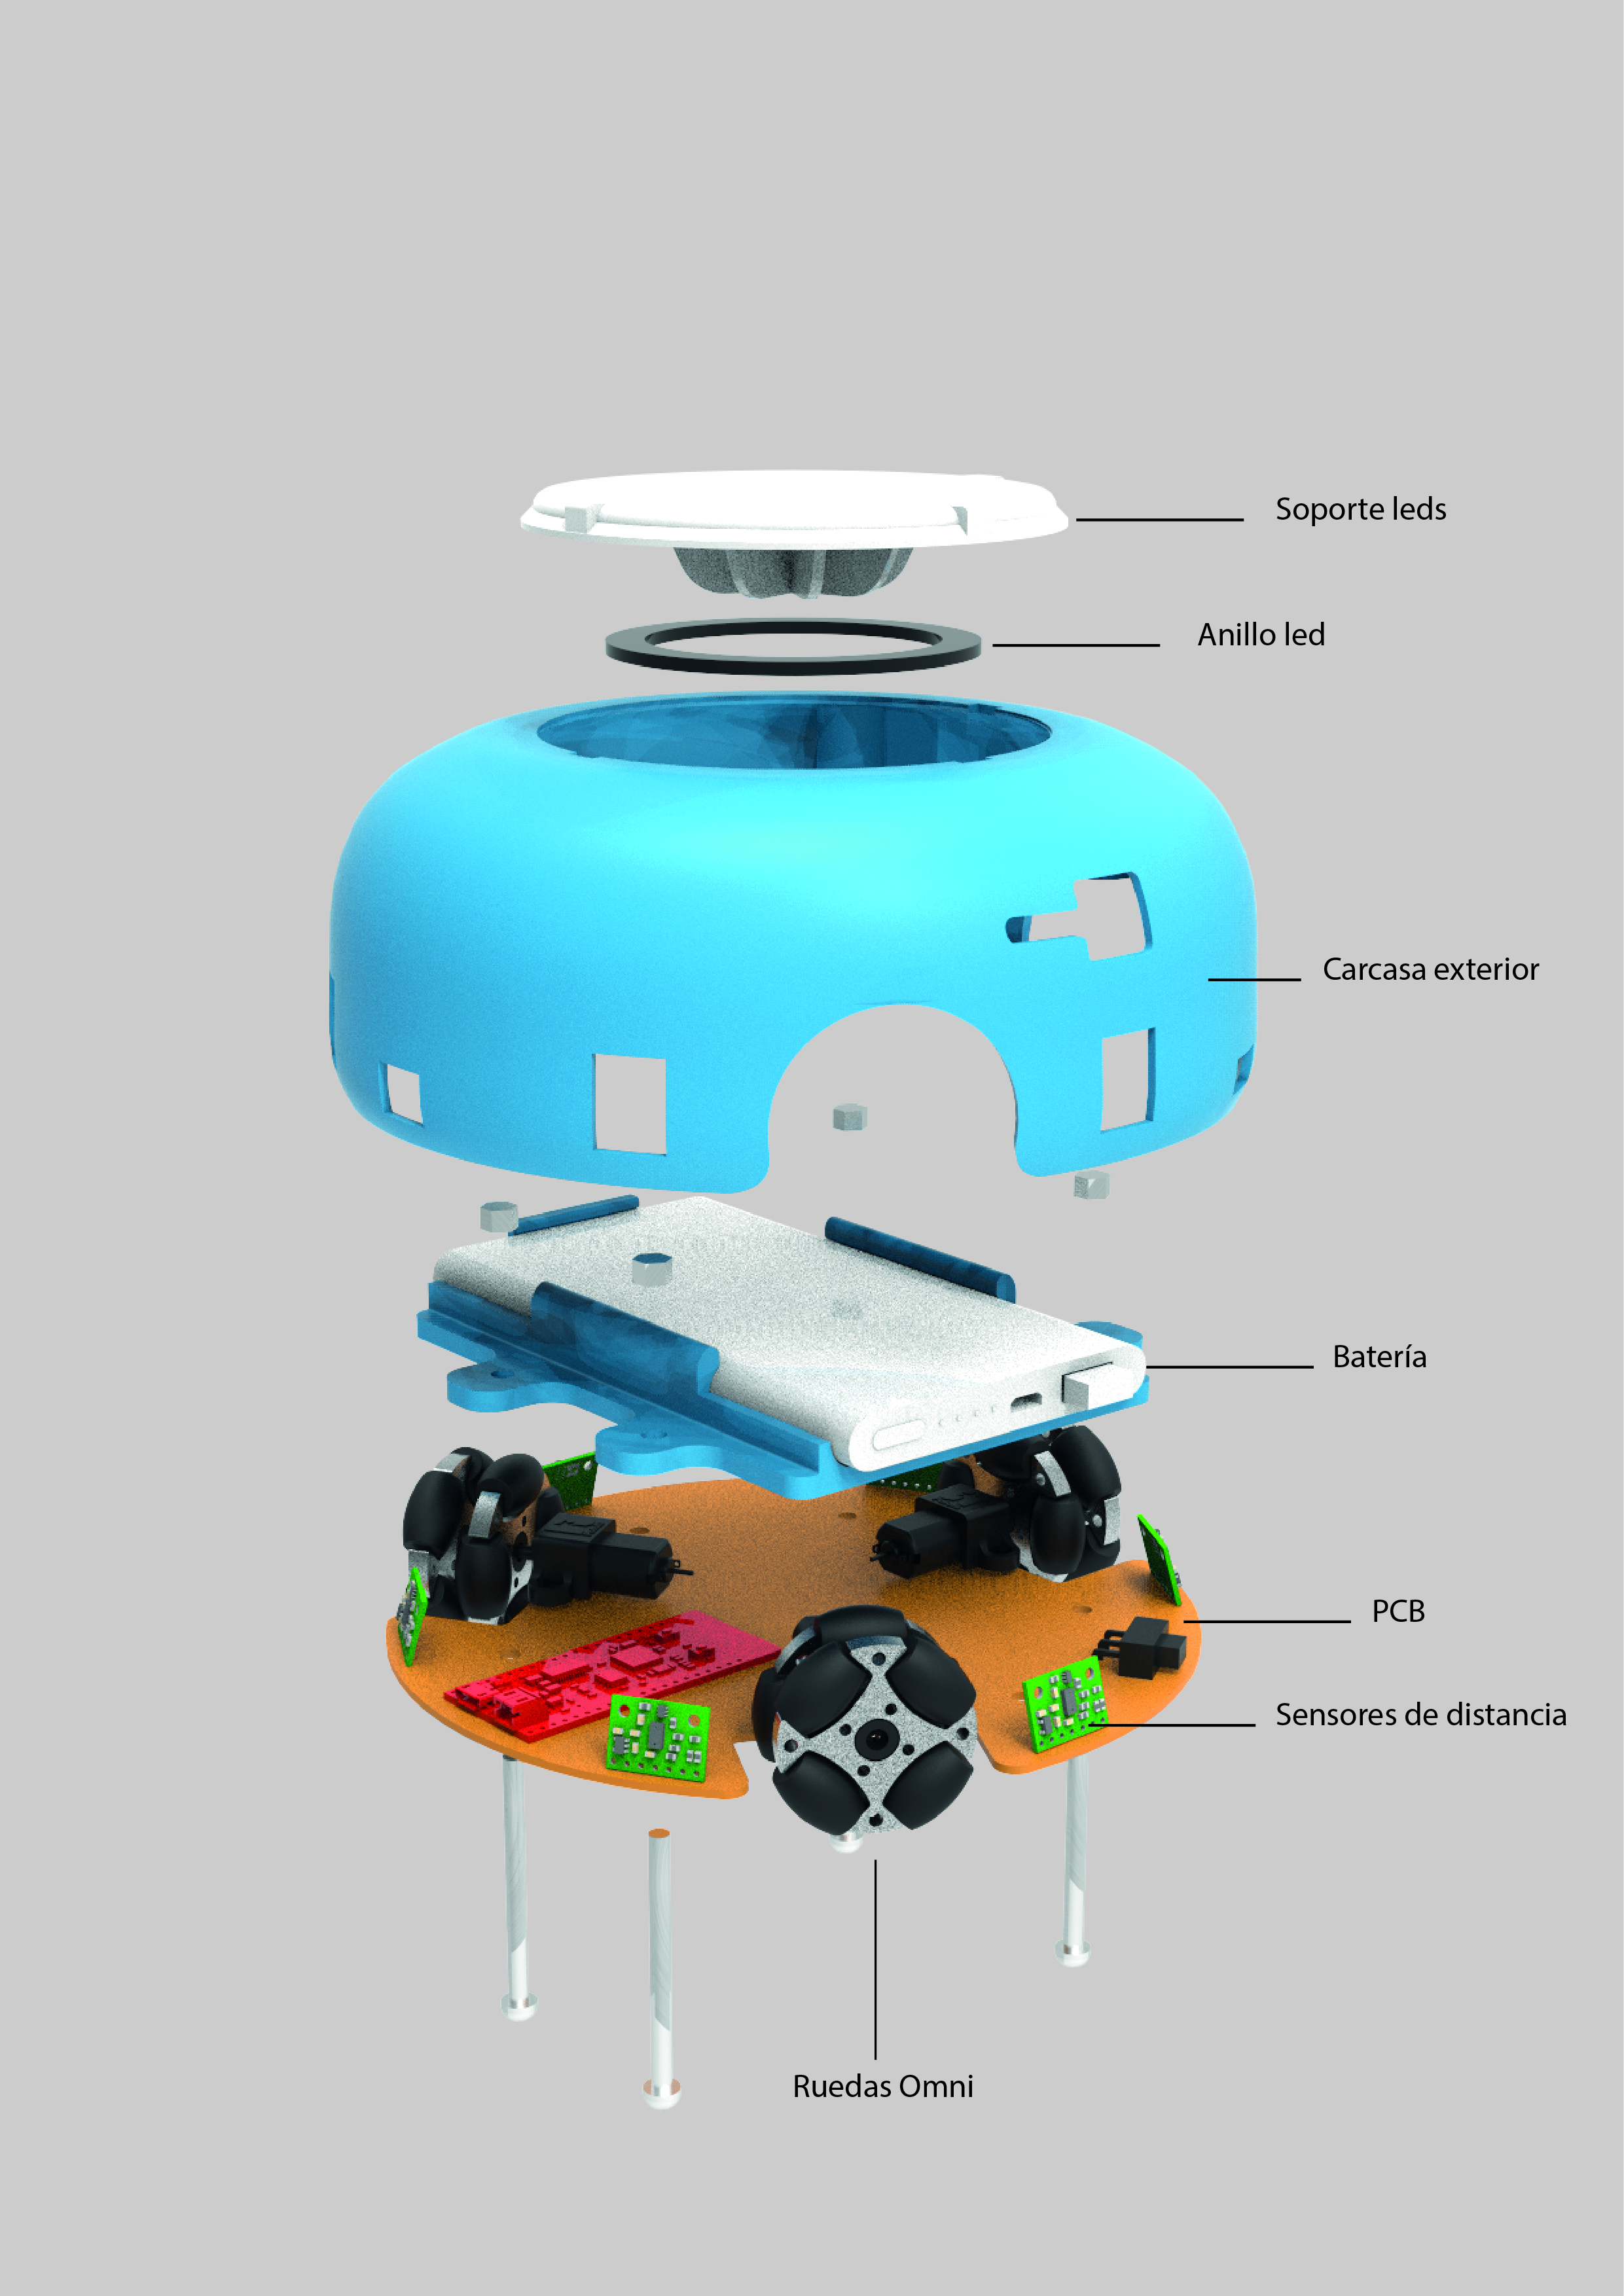
\includegraphics[width=\textwidth]{render-componentes.png}
			\end{center}
		\end{column}
	\end{columns}
\end{frame}

 \begin{frame}
 	\frametitle{Plan de intervención}
 	\begin{itemize}
 		\item Familiarización con el robot
 		\item Exploración
 		\item Incorporación de objetos
 		\item Secuenciación de movimientos
 		\item Resolución de problemas	.
 	\end{itemize}
 \end{frame}
 
\begin{frame}	
\Huge{\centerline{Preguntas}}
\end{frame}

%------------------------------------------------

\begin{frame}
\frametitle{Lecturas Recomendadas}
\footnotesize{

\begin{thebibliography}{99} % Beamer does not support BibTeX so references must be inserted manually as below
\bibitem{butia} Proyecto Butiá.
\newblock Página del proyecto Butiá.
\newblock\emph{www.fing.edu.uy/inco/proyectos/butia}. 2018.

\bibitem{MINA} Grupo MINA.
\newblock Página del grupo MINA.
\newblock\emph{www.fing.edu.uy/inco/grupos/mina}. 2018.

\bibitem{CICEA} CICEA.
\newblock Página del Centro Interdisciplinario en Cognición para la Enseñanza y el Aprendizaje.
\newblock\emph{www.cicea.ei.udelar.edu.uy}. 2018.

\end{thebibliography}
}
\end{frame}

%----------------------------------------------------------------------------------------

\end{document}
